\documentclass[12pt]{article}

\usepackage[ngerman]{babel}
\usepackage{titlesec}
\usepackage{graphicx}
\usepackage{textcomp}
\usepackage[a4paper, lmargin=2.5cm, rmargin=2.5cm, top=2.5cm, bottom=3cm]{geometry}
\usepackage{setspace}
\usepackage{amsmath}
\usepackage{amsfonts}
\usepackage{amssymb}
\usepackage{amsthm}
\usepackage[utf8]{inputenc}
\usepackage{stmaryrd}
\usepackage{bibgerm}
\usepackage{caption}
\usepackage{aligned-overset}
\usepackage{subcaption}
\usepackage[utf8]{inputenc}
\pagestyle{plain}
\pagenumbering{arabic}
\usepackage[square,sort,comma,numbers]{natbib}

\usepackage{xcolor}
\usepackage[framemethod,tikz]{mdframed}
\usetikzlibrary{shadows}

\mdfdefinestyle{outer}{outerlinewidth=0.5pt,backgroundcolor=blue!5,roundcorner=10pt,outerlinecolor=blue,innerlinewidth=0.5pt,innerlinecolor=black}
\mdfdefinestyle{inner}{leftmargin=0.1cm,rightmargin=0.1cm,outerlinewidth=0.5pt,innerlinewidth=0.5pt,innerlinecolor=black,outerlinecolor=black,backgroundcolor=lightgray!10,roundcorner=5pt,linecolor=black}

\newcommand{\qenc}{q_{\boldsymbol\phi}(\mathbf{z}|\mathbf{x}_i)}
\newcommand{\penc}{p_{\boldsymbol\theta}(\mathbf{z}|\mathbf{x}_i)}
\newcommand{\pdec}{p_{\boldsymbol\theta}(\mathbf{x}_i|\mathbf{z})}
\newcommand{\E}{\mathbb{E}}
\newcommand{\z}{\mathbf{z}}
\newcommand{\x}{\mathbf{x}_i}
\DeclareMathOperator*{\argmin}{arg\,min}
\newtheorem{theorem}{Theorem}
\allowdisplaybreaks

\begin{document}
	\setlength{\parindent}{0em}
	\onehalfspacing
\begin{titlepage}
	\begin{center}
		\huge\textbf{Missing Data Imputation mit \\Variational Autoencodern}\\
		\vspace{1.5cm}
		\LARGE\textbf{{Projektarbeit}}\\
		\vspace{0.5cm}
		\normalsize
		Im Rahmen der Vorlesung\\
		Stochastic Machine Learning\\
		\vspace{0.3cm}
		vorgelegt am 10. Februar 2021 \\
		\vspace{0.7cm}
		
		\begin{figure}[h!]
			\centering
			
\includegraphics[scale=0.4]{Unifreiburg}
		\end{figure}
	
		\vspace{0.7cm}
		\large \textbf{Albert-Ludwigs-Universität Freiburg}\\
   		\vspace{0.2cm}
		\large {Institut für Mathematik}\\
		\vspace{1cm}
		\large {Niklas Brunn}\\
		\large {Ben Deitmar}\\
		\large {Sebastian Hahn}\\
		\large {Jannis Klingler}\\
		\large {Clemens Schächter}\\

		\vspace{1.8cm}
	\end{center}
\end{titlepage}

	\tableofcontents
	\newpage
	\section[Einleitung]{Einleitung}
	Der \emph{Variational Autoencoder} (kurz: VAE) ist ein unsupervised Deep-Learning Algorithmus, welcher es ermöglicht niedrigdimensinale latente Darstellungen aus hochdimensionales Daten zu erlernen. Nach der Trainingsphase kann der VAE schließlich als probabilistisches Generatives Modell zum erzeugen neuer Daten verwendet werden.\\
	Da das Modell selbst erlernen muss, 
	wie die Datenpunkte am besten gruppiert werden, wird auch das Erkennen unbekannter Eigenschaften ermöglicht.\\
	Beim generieren von Bildern wie menschlichen Gesichtern kann die Performance dabei durchaus mit state-of-the-art Modellen wie Genrative Adversarial Networks mithalten. Die Anwendungsmöglichkeiten des Modells sind vielseitig, so werden VAEs unter anderem zum Modellieren chemischer Moleküle, zur Verarbeitung menschlicher Sprache oder zum erkennen beschädigter Daten und Schätzung von Unsicherheit eingesetzt.\\
	Im Rahmen dieser Projektarbeit wollen wir Variational Autoencoder darauf trainieren Vorhersagen für hochdimensionale Daten mit zeitlicher Abhängigkeit, sogenannten \emph{Time Series} zu treffen. Hierbei 
	spezialisieren wir uns auf Serien von Bildern und 
	konzentrieren uns zunächst auf das Rekonstruieren beschädigter Daten bzw. fehlender Datenpunkte. \\
	Da dem \emph{Variational Autoencoder} die Annahme zugrunde liegt, dass die Verteilung der Datenpunkte 
	unabhängig und identisch verteilt ist, ist eine Anwendung auf unsere Problemstellung nicht ohne weitere 
	Anpassungen sinnvoll.\\
	Ein recht trivialer Ansatz hierfür ist es, die zeitliche Komponente in den Daten zu 
	vernachlässigen und die gesamte Time Series dem VAE zusammengefasst als einen Datenvektor zu übergeben. Wenn der Trainingsdatensatz unbeschädigt ist, wird der beschädigten Time Series die latente Darstellung zugewiesen, die einer unbeschädigten Time Series am nächsten kommt. Vom Decoder wird die Time Series nun vollständig rekonstruiert, da ihm beschädigte Daten nach dem Trainingsprozess unbekannt sind.\\
	Ein weiterer Ansatz ergibt sich, wenn man die zeitlichen Zusammenhänge der Time Series 
	im Latenten Raum linear interpoliert. Hier bilden die einzelnen Frames der Time Series unseren Trainingsdatensatz. Durch lineare Interpolation lassen sich die Übergänge nun auch in stetiger Zeit modellieren. \\
	Wie wir sehen werden, können beide Ansätze jedoch auf etwas komplexeren Datensätzen keine zufriedenstellende Ergebnisse mehr liefern.
	Eine Möglichkeit diese komplexen Zusammenhängen zwischen den Zeitschritten in \emph{time series} besser zu erlernen bietet der \emph{Ordinary Differential Equation Variational Auto-Encoder} (kurz: ODE$^2$-VAE). Die zeitlichen Abhängigkeiten unter den Datenpunkten werden hier mit Differentialgleichungen zweiter Ordnung modelliert, welche im Trainingsprozess erlernt werden. Schon nur aus drei Inputbildern kann die gesamte Time Series in stetiger Zeit rekonstruiert werden.\\
	\textbf{TODO: Einleitung SDE-VAE}
	\\
	\\
	In dieser Arbeit werden wir in einem theoretischen Teil die mathematischen Grundlagen einführen, auf denen der Variational Autoencoder und der ODE$^2$-VAE aufbauen.\\ 
	In einem praktischen Teil werden schließlich Anwendungsmöglichkeiten der beiden Modelle auf unsere Problemstellung präsentiert.\\
	Dabei wird sowohl auf die Implementierung der
	theoretischen Resultate, als auch auf die experimentellen Ergebnisse eingegangen.\\
	Die in dieser Arbeit verwendeten Quellen sind die Paper \emph{Auto-Encoding Variational Bayes} \cite{vae}, sowie \emph{An Introduction to Variational Autoencoders}, \cite{intvae} beide von Diederik P. Kingma und Max Welling und \emph{ODE$^{\ 2}$-VAE: Deep generative second order ODEs with Bayesian neural networks} \cite{ode2vae} von Ç. Yıldız, M. Heinonen und H. Lähdesmäki.
	\newpage
	
	\section[Theoretische Ausarbeitung]{Theoretische Ausarbeitung}
	Angenommen wir haben einen Datensatz $\textbf{X} = \lbrace\x \rbrace_{i=1}^{N}$, der aus $N$ unterschiedlichen i.i.d. verteilten Datenpunkten $\x\sim p(\x)$ besteht, welche hochdimensionale Realisierungen einer unbekannten Zufallsvariable sind.\\
	Um den Prozess, der die Daten erzeugt besser modellieren und später erlernen zu können, werden sogenannte \emph{latenten Variablen} $\z$ eingeführt. Diese sind stetige und nicht beobachtbare Zufallsvariablen, welche die Eigenschaften des Bildes festlegen, die es charakterisiert.  \\
	Der sogenannte \emph{latente Raum} $\mathcal{Z}$, über den die latenten Variablen $\z$ definiert sind, ist nach Wahl von viel geringerer Dimension als der Raum $\mathcal{X}$ der ursprünglichen Verteilung.\\
	Schauen wir uns einmal an, wie die Datenpunkte des Datensatzes in einem solchen latenten Variablen Modell entstehen.\\
	Zuerst wird eine latente Darstellung $\z \sim  p(\z)$  gezogen. Mit dieser wird  $\x \sim  p(\x|\z)$ nun durch eine bedingte Verteilung ermittelt. So lässt sich nun die Dichtefunktion von $p(\x)$ über Marginalisierung durch ein Integral über alle latenten Werte beschreiben.
	\begin{align*}
	p(\x)= \int_{\z} p(\x,\z) d\textbf{z} = \int_{\z} p(\x|\z)p(\z) d\z
	\end{align*}
	Dieses Integral ist jedoch unberechenbar und kann aufgrund der hohen Dimension des Raumes $\mathcal{X}$ in der Regel auch nicht sinnvoll approximiert werden. 
	Die bedingte Verteilung $p(\z|\x)$, mit welcher sich für Datenpunkte $\x$ eine zugehörige latente Darstellung $\z$ finden lässt, ist ebenfalls nicht berechenbar. Dies und die Unberechenbarkeit der marginalen Wahrscheinlichkeit impliziert sich durch den Satz von Bayes gegenseitig: 
	\begin{align*}
	p(\z|\x)= \frac{p(\x|\z)p(\z)}{p(\x)}
	\end{align*}
	Die gemeinsame Verteilung $p(\x,\z) = p(\x|\z)p(\z)$ lässt sich anhand der Daten approximieren, dabei sind die Datenpunkte Realisierungen dieser Verteilung. Wäre $p(\x)$ beobachtbar, könnten wir auch $p(\z|\x)$ errechnen. Eine Umkehrung dieser Überlegung gilt ebenfalls. \\ 
	
	Die Verteilungen $p(\x|\z),\ p(\z|\x),\ p(\z)$ und $p(\x)$ fassen wir als durch ${\boldsymbol\theta}$ parametrisierte Familien auf. Für die optimalen Parameter $\boldsymbol\theta^{*}$ soll dabei gelten $p_{\boldsymbol\theta^{*}}(\x) \approx p(\x)$.\\
	Weiter führen wir wegen der Unberechenbarkeit von $p_{\boldsymbol\theta}(\z|\x)$ das Inferenzmodell $q_{\boldsymbol\phi}(\z|\x)$ ein und suchen die Parameter $\boldsymbol\phi^{*}$ für die $q_{\boldsymbol\phi^{*}}(\z|\x) \approx p_{\boldsymbol\theta}(\z|\x)$ gilt.\\ 
	Mit einem Variational Autoencoder werden die Verteilungen $q_{\boldsymbol\phi}(\z|\x)$ und $p_{\boldsymbol\theta}(\x|\z)$ durch neuronale Netze dargestellt und approximiert.\\
	Im AEVB-Algorithmus (kurz für \emph{Auto-Encoding Variational Bayes}) können die geeigneten Parameter $\boldsymbol\phi^{*}$ und $\boldsymbol\theta^{*}$ gemeinsam erlernt werden.
	\subsection[VAE]{AEVB-Algorithmus und Variational Autoencoder}
	Wir betrachten dafür für einen beliebigen Datenpunkt $\x \in \mathbf{X}$ die Reverse KL-Divergenz der Approximation $\qenc$ nach $\penc$:
	\begin{align*}
	D_{KL}\big[\qenc || \penc\big] \overset{\text{Def.}}&{=} \E_{\z\sim q_{\boldsymbol\phi}}\left[\log\left(\frac{\qenc}{\penc}\right)\right] \\
	\overset{\text{Bayes}}&{=} \E_{\z\sim q_{\boldsymbol\phi}}\left[\log\left(\frac{p_{\boldsymbol\theta}(\x)\qenc}{
		\pdec p_{\boldsymbol\theta}(\z)}\right)\right]\\
	&=\E_{\z\sim q_{\boldsymbol\phi}}\left[\log\big(p_{\boldsymbol\theta}(\x)+\log\left(\frac{\qenc}{p_{\boldsymbol\theta}(\z)} \right) -\log\big(\pdec\big)\right]\\
	&=\log\big(p_{\boldsymbol\theta}(\x)\big) + D_{KL}\big[\qenc||p_{\boldsymbol\theta}(\z)\big]-\E_{\z\sim q_{\boldsymbol\phi}}\big[\log\big(\pdec\big)\big]
	\end{align*}
	Durch Äquivalenzumformung erhalten wir schließlich:
	\begin{align*}
	\log\big(p_{\boldsymbol\theta}(\x)\big) - \underbrace{D_{KL}\big[\qenc || \penc\big]}_{\ge 0} =\underbrace{ \E_{\z\sim q_{\boldsymbol\phi}}\big[\log\big(\pdec\big)\big] - D_{KL}\big[\qenc||p_{\boldsymbol\theta}(\z)\big]}_{=:\ \mathrm{ELBO}\ =\ -\mathcal{L}(\boldsymbol\theta,\boldsymbol\phi,\mathbf{x}_i)}
	\end{align*}
	Die rechte Seite wird auch \emph{Evidence Lower Bound} (kurz: ELBO) genannt und dient als (negative) Verlustfunktion des Variational Autoencoder. Als untere Schranke der Loglikelihood führt eine Maximierung der ELBO dazu, dass zum einen die Reverse KL-Divergenz der Approximation zur wahren Verteilung verringert wird, was eine immer besser werdende Beschreibung von $\penc$ durch $\qenc$ impliziert und zum anderen die Likelihood Daten des Datensatzes zu erzeugen groß wird.\\
	Wir haben in $\mathcal{L}(\boldsymbol\theta,\boldsymbol\phi,\x)$ also eine zur Minimierung geeignete Funktion gefunden und wollen einen geeigneten Algorithmus verwenden, der uns das Finden der optimalen Parameter
	\begin{align*}
	\boldsymbol\theta^{*},\boldsymbol\phi^{*} = \argmin_{\boldsymbol\theta,\boldsymbol\phi} \mathcal{L}(\boldsymbol\theta,\boldsymbol\phi,\x).
	\end{align*}
	in einer angemessenen Berechnungsdauer ermöglicht. Dazu müssen während des Lernprozesses die Gradienten bezüglich der Parameter berechnet werden.
	\begin{align*}
	\nabla_{\boldsymbol\theta,\boldsymbol\phi} \mathcal{L}(\boldsymbol\theta,\boldsymbol\phi,\x) = \nabla_{\boldsymbol\theta,\boldsymbol\phi} \Bigl[D_{KL}\big[\qenc || p_{\boldsymbol\theta}(\textbf{z})\big]\Bigl]- \nabla_{\boldsymbol\theta,\boldsymbol\phi}\Bigl[\mathbb{E}_{\z\sim q_{\boldsymbol\phi}}\big[\log\big(\pdec\big)\big]\Bigl] 
	\end{align*}
	Die KL-Divergenz ist in vielen Fällen mit analytischen Methoden berechen- und differenzierbar, genauer betrachtet werden muss aber der Gradient des Erwartungswertes bezüglich $\boldsymbol\phi$. \\
	Gegeben $\textbf{x}_{i}$ ist die latente Darstellung $\z$ kein deterministisch festgelegter Wert, sondern wird durch die von diesen Parametern abhängige Verteilung $\z \sim \qenc$ bestimmt. Da der Gradient später durch Backpropagation berechnet wird, müssen auch die Layer durchschritten werden, die diesen Zufallsprozess enthalten. Monte-Carlo Schätzungen sind außerdem nicht immer mit zufriedenstellender Genauigkeit möglich, denn der Gradient des Erwartungswertes lässt sich in der Regel nicht zu einem neuen Erwartungswert umschreiben, da die Dichtefunktion von $\boldsymbol\phi$ abhängig ist.
	\begin{align*}
	\nabla_{\boldsymbol\phi}\Bigl[\mathbb{E}_{\z\sim q_{\boldsymbol\phi}}\big[\log\big(\pdec\big)\big]\Bigl] &= \nabla_{\boldsymbol\phi} \int_{\textbf{z}}\qenc\log\big(\penc)\big)d\textbf{z} \notag \\
	&= \int_{\textbf{z}}\nabla_{\boldsymbol\phi}\qenc\log\big(\pdec)\big)d\textbf{z}  
	\end{align*}
	
	Der \emph{Reparametrisierungs Trick} bietet eine Lösung für diese Problematik. \cite{repara}
	Wir reparametrisieren die latente Variable $\textbf{z} = g_{\boldsymbol\phi}(\boldsymbol\epsilon,\textbf{x}_{i})$ mit einer differenzierbaren, durch $\boldsymbol\phi$ parametrisierten Funktion $g$ und einer Zufallsvariablen $\boldsymbol\epsilon \sim p(\boldsymbol\epsilon)$, deren Dichtefunktion jedoch nicht von $\boldsymbol\phi$ abhängig ist. Somit erhalten wir nach Anwendung
	\begin{align*}
	\nabla_{\boldsymbol\phi}\Bigl[\mathbb{E}_{\z\sim q_{\boldsymbol\phi}}\big[\log\big(\pdec\big)\big]\Bigl] &= \nabla_{\boldsymbol\phi}\Bigl[\mathbb{E}_{\boldsymbol\epsilon\sim p(\boldsymbol\epsilon)}\big[\log\big(p_{\boldsymbol\theta}(\textbf{x}_{i}|g_{\boldsymbol\phi}(\boldsymbol\epsilon,\textbf{x}_{i}))\big)\big]\Bigl] \notag\\
	&= \nabla_{\boldsymbol\phi} \int_{\boldsymbol\epsilon}p(\boldsymbol\epsilon)\log\big(p_{\boldsymbol\theta}(\textbf{x}_{i}|g_{\boldsymbol\phi}(\boldsymbol\epsilon,\textbf{x}_{i}))\big)d\boldsymbol{\epsilon} \notag \\
	&=  \int_{\boldsymbol\epsilon}p(\boldsymbol\epsilon)\nabla_{\boldsymbol\phi}\log\big(p_{\theta}(\textbf{x}_{i}|g_{\boldsymbol\phi}(\boldsymbol\epsilon,\textbf{x}_{i}))\big)d\boldsymbol{\epsilon} \notag \\
	&=\mathbb{E}_{\epsilon\sim p(\boldsymbol\epsilon)}\big[\nabla_{\boldsymbol\phi}\log\big(p_{\boldsymbol\theta}(\textbf{x}_{i}|g_{\boldsymbol\phi}(\boldsymbol\epsilon,\textbf{x}_{i}))\big)\big] \notag \\
	\overset{\text{M.C.}}&{\simeq} \frac{1}{L}\sum_{l=1}^{L}\nabla_{\boldsymbol\phi}\log\big(p_{\boldsymbol\theta}(\textbf{x}_{i}|g_{\boldsymbol\phi}(\boldsymbol\epsilon_{l},\textbf{x}_{i}))\big).
	\end{align*}
	Was eine Berechnung der Gradienten, sowie Monte-Carlo-Schätzung des Erwartungswertes ermöglicht.\\
	Die negative ELBO soll in unserem gesuchten Algorithmus nicht nur für einen einzigen Datenpunkt $\textbf{x}_{i}$, sondern vielmehr auf dem gesamten Datensatz $\textbf{X}$, also für alle $\textbf{x}_{i}$ minimiert werden, denn wir haben
	\begin{align*}
	\log\big(p_{\boldsymbol\theta}(\textbf{X})\big)&=\log\big(p_{\boldsymbol\theta}(\textbf{x}_{1},\ldots,\textbf{x}_{N})\big)\overset{\text{i.i.d.}}{=}\log\left(\prod_{i=1}^{N}p_{\boldsymbol\theta}(\x)\right) =\sum_{i=1}^{N}\log\big(p_{\boldsymbol\theta}(\x)\big) \notag \\&= \sum_{i=1}^{N} D_{KL}\big[\qenc||\penc\big] -
	\mathcal{L}(\boldsymbol\theta,\boldsymbol\phi,\x).
	\end{align*}
	 
	Der kürzeren Berechnungsdauer geschuldet, werden dafür Minibatches $\textbf{M} = \{\textbf{x}_{i}\}_{i=1}^{M} \subset \textbf{X}$ gezogen und die ELBO nur auf diesen optimiert.
	\begin{align*}
	&\mathcal{L}(\boldsymbol\theta,\boldsymbol\phi,\textbf{X}) \simeq \mathcal{L}(\boldsymbol\theta,\boldsymbol\phi,\textbf{M}) = \mathbb{E}\lbrack\mathcal{L}(\boldsymbol\theta,\boldsymbol\phi,\textbf{x}_{i})\rbrack \simeq \frac{N}{M}\sum_{i=1}^{M}\mathcal{L}(\boldsymbol\theta,\boldsymbol\phi,\textbf{x}_{i})\\
	&\simeq \frac{N}{M}\sum_{i=1}^{M}  \left(D_{KL}\big[\qenc||p_{\boldsymbol\theta}(\z)\big] - \frac{1}{L}\sum_{l=1}^{L}\log\big(p_{\boldsymbol\theta}(\textbf{x}_{i}|g_{\boldsymbol\phi}(\boldsymbol\epsilon_{l},\textbf{x}_{i}))\big)\right)
	\end{align*}
	
	Experimentell hat sich gezeigt, dass ein groß gewähltes $M$, z.B. $M=100$ es zulässt die Anzahl der Stichproben von $\boldsymbol\epsilon$ für die Monte-Carlo Schätzung des Erwartungswertes $\mathbb{E}_{\boldsymbol\epsilon\sim p(\boldsymbol\epsilon)}\big[\log\big(p_{\boldsymbol\theta}(\textbf{x}_{i}|g_{\boldsymbol\phi}(\boldsymbol\epsilon,\textbf{x}_{i}))\big)\big]$ als $L=1$ zu wählen.
	\\
	Wir erhalten den AEVB-Algorithmus \emph{(Auto Encoding Variational Bayes)}: \\
	
	\hrule
	\vspace{0,15cm}
	\textbf{AEVB-Algorithmus}
	\vspace{0,05cm}
	\hrule
	\vspace{0,20cm}
	\textbf{1)}  $\boldsymbol\phi,\boldsymbol\theta \leftarrow$ Ziehe die Parameter zufällig.\\
	\textbf{2)} $\mathbf{M} \leftarrow$ Ziehe ein Minibatch $\textbf{M} = \{\textbf{x}_{i}\}_{i=1}^{M}$ mit $|\textbf{M}| \ge 100$. \\
	\textbf{3)} $\boldsymbol\epsilon \leftarrow$ Ziehe einen Wert für $\boldsymbol\epsilon \sim p(\boldsymbol\epsilon)$.\\
	\textbf{4)} $\mathbf{g} \leftarrow$ Berechne die Gradienten $\nabla_{\boldsymbol\theta,\boldsymbol\phi} \mathcal{L}(\boldsymbol\theta,\boldsymbol\phi,\textbf{M})$. \\
	\textbf{5)} $\boldsymbol\phi,\boldsymbol\theta \leftarrow$ Aktualisiere die Parameter.\\
	\textbf{6)} Wiederhole ab Schritt \textbf{2)}, bis zur Konvergenz des Verfahrens.
	\vspace{0,05cm}
	\hrule
	\vspace{0,3cm}
	\ \\
	Beim Variational Autoencoder werden die Verteilungen $\qenc$ und $\pdec$ durch Neuronale Netze mit den Parametern $\boldsymbol\theta$ und $\boldsymbol\phi$ approximiert und durch den AEVB-Algorithmus trainiert. In diesem Kontext wird $\pdec$ auch \emph{probabilistischer Decoder} genannt und $\qenc$ \emph{probabilistischer Encoder}. \\
	Nach der Trainingsphase können Decoder und Encoder jedoch voneinander getrennt werden. Mit dem Decoder lassen sich nun neue Daten erzeugen, indem hypotetische latente Darstellungen als Input genutzt werden.\\
	Für das Inferenzmodell $\qenc$ wird in einem Variational Autoencoder häufig (aber nicht zwingenderweise) eine Multivariate Normalverteilung $\mathcal{N}(\boldsymbol\mu_{i},\boldsymbol\sigma_{i}^{2}\mathbf{I})$ mit diagonaler Kovarianzmatrix gewählt. \\
	Hier bildet
	der Encoder einen Input $\textbf{x}_{i}$ auf den Lageparameter $\boldsymbol\mu_{i}$ und den Streuungsparameter $\boldsymbol\sigma_{i}$ ab. Diese Parameter sind deterministische Funktionswerte des Encodernetzwerkes, es gilt also $\boldsymbol\mu_{i} = \boldsymbol\mu_{\boldsymbol\phi}(\textbf{x}_{i})$ und $\boldsymbol\sigma_{i} = \boldsymbol\sigma_{\boldsymbol\phi}(\textbf{x}_{i})$.\\ 
	Auf diesen Output wird der Reparametrisation Trick angewandt, um die Berechnung des Gradienten mit Backpropagation zu ermöglichen.\\
	Gegeben ein Datenpunkt $\textbf{x}_{i}$ erhalten wir eine latente Darstellung deshalb durch $\textbf{z} = g_{\boldsymbol\phi}(\boldsymbol\epsilon,\textbf{x}_{i})  =\boldsymbol\mu_{\boldsymbol\phi}(\textbf{x}_{i}) +\boldsymbol\sigma_{\boldsymbol\phi}(\textbf{x}_{i}) \odot \boldsymbol\epsilon$ mit $\boldsymbol\epsilon \sim p(\boldsymbol\epsilon) = \mathcal{N}(\textbf{0},\textbf{I})$. Hierbei steht $\odot$ für eine elementweise Multiplikation der beiden Vektoren.\\
	Die Verteilung $p_{\boldsymbol\theta}(\z)$ wird als multivariate Standardnormalverteilung $\mathcal{N}(\mathbf{0},\mathbf{I})$ festgelegt und nicht durch ein Neuronales Netz dargestellt. Interessanterweise ist diese Wahl einer parameterfreien, recht einfachen Verteilung möglich. Es lässt sich durch Abbilden von Realisierungen einer multivariat standardnormalverteilten Zufallsvariable tatsächlich eine beliebige andere Verteilung erzeugen. 
	\vspace*{0.1cm}
	\begin{figure}[h!]
	\centering
	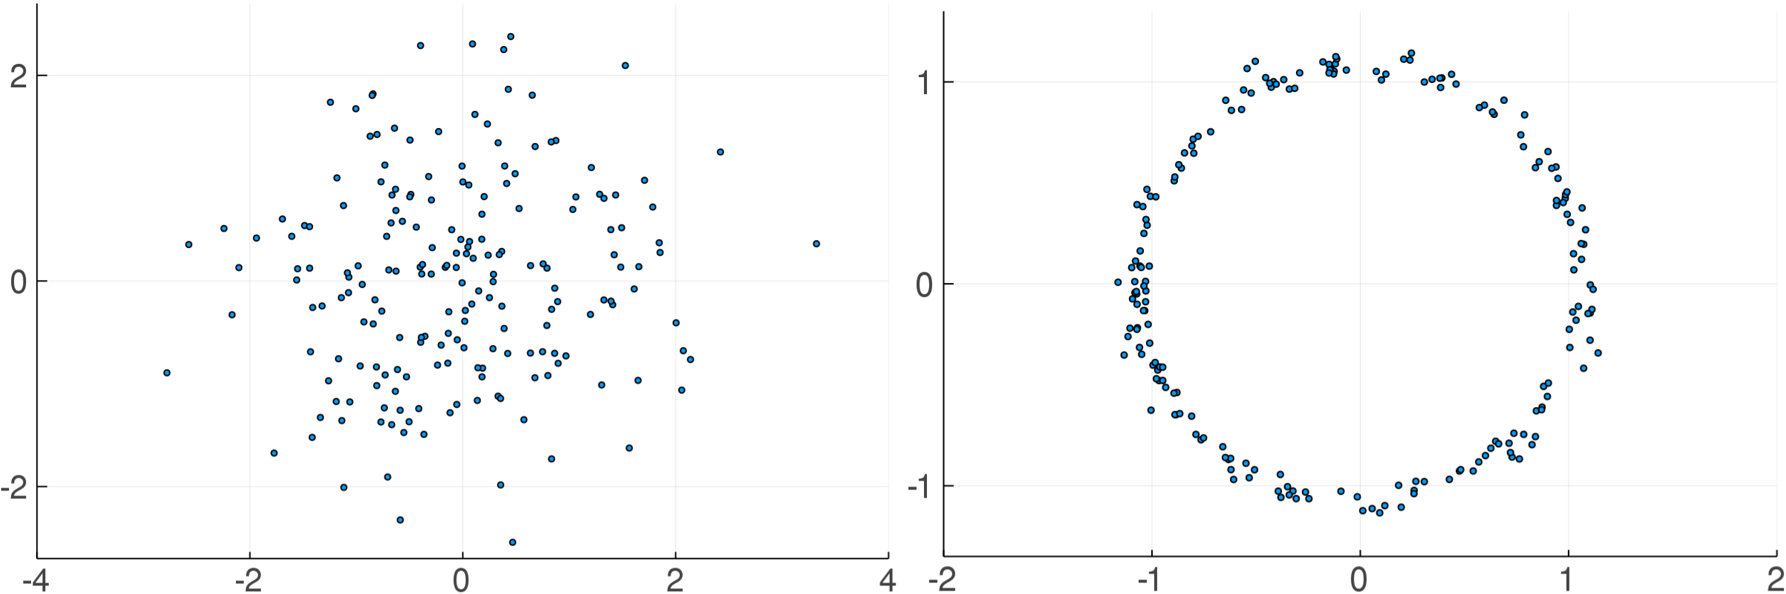
\includegraphics[scale=0.4]{normalverteilt}
	\captionsetup{labelformat=empty}
	\caption{Gegeben die Realisierungen einer Zufallsvariablen $\z\sim \mathcal{N}(\mathbf{0},\mathbf{I})$  (Links) lässt sich mit Abbildung durch eine Funktion, hier $g(\textbf{z})= \frac{\textbf{z}}{15}+\frac{\textbf{z}}{||\textbf{z}||}$ eine ganz andere Verteilung erzeugen (Rechts). Dies nutzt der VAE aus, um aus Realisierungen einer normalverteilten Zufallsvariablen komplexe Verteilungen in großer Dimension zu modellieren. Die Funktion g, beim VAE der Decoder wird aus den Daten erlernt. \textbf{}\cite{tutvae}}
	\end{figure}
	
	Welche Verteilung für den Decoder $\pdec$ dafür am besten geeignet ist, hängt vom Typ der zu erzeugenden Daten ab.\\ Für binäre Daten  $\textbf{x}_{i} \in \{0,1\}^{P}$ werden wir eine multivariate Bernoulliverteilung verwenden, also $p_{\theta}(\textbf{x}_{i}|\textbf{z}) =  \mathcal{B}(\boldsymbol{p}_{i})$. Gemeint ist hiermit eine elementweise Auswertung univariater Bernoulliverteilungen.\\
	Für stetige Daten $\textbf{x}_{i} \in \mathbb{R}^{P}$ wählen wir eine multivariate Normalverteilung $p_{\theta}(\textbf{x}_{i}|\textbf{z}) = \mathcal{N}(\boldsymbol{\hat{\mu}}_{i},\boldsymbol{\hat{\sigma}}_{i}^{2}\textbf{I})$.\\
	Hierbei sind $\boldsymbol{\hat{\mu}}_{i} = \boldsymbol{\hat{\mu}}_{\boldsymbol\theta}(\textbf{z})$ und $\boldsymbol{\hat{\sigma}}_{i}^{2} = \boldsymbol{\hat{\sigma}}_{\boldsymbol\theta}^{2}(\textbf{z}) $ bzw. $\textbf{p}_{i} = \textbf{p}_{\boldsymbol\theta}(\textbf{z})$ die Ausgaben des Decodernetzwerkes.\newpage
	\begin{figure}[h!]
	\centering
	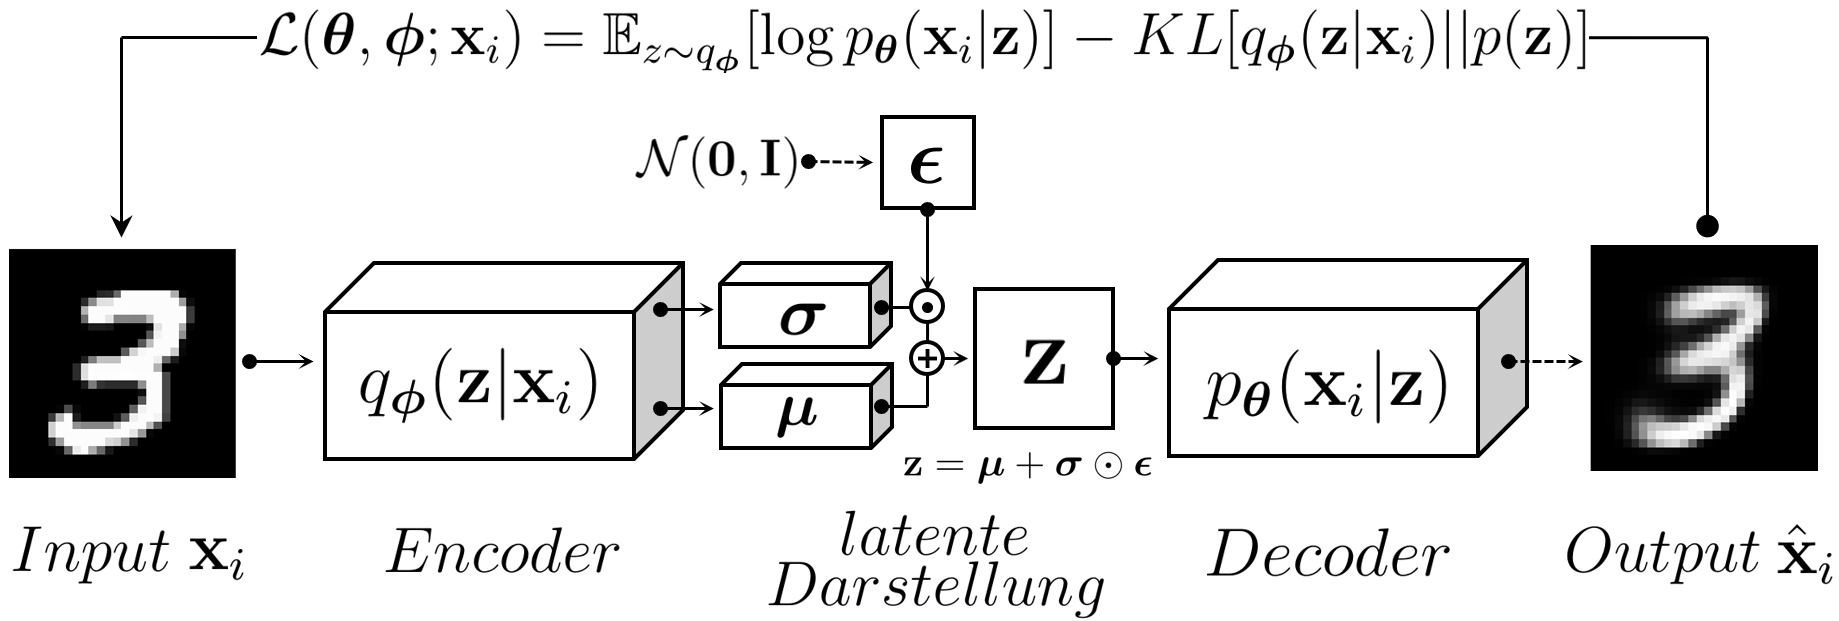
\includegraphics[scale=0.41]{VAE-Modell}
	\captionsetup{labelformat=empty}
	\caption{Schematische Darstellung eines Variational Autoencoders. Der hochdimensionale Input $\mathbf{x}_i$ wird durch den Encoder auf einen Erwartungswertvektor $\boldsymbol{\mu}$ und Streuungsparameter $\boldsymbol{\sigma}$ abgebildet. Anschließend wird eine niedrigdimensionale latente Darstellung \textbf{z} gezogen. Dabei wird der Reparametrisierungstrick $\textbf{z}=\boldsymbol{\mu}+\boldsymbol{\sigma} \odot \boldsymbol{\epsilon}$ angewandt. Der Decoder rekonstruiert nun mit dieser Darstellung einen Output $\hat{\mathbf{x}}_i$. Der Modellverlust ist durch die negative ELBO gegeben, durch Minimierung dieser kann das Modell optimiert werden.\\}
	\centering
	\begin{minipage}{.5\textwidth}
		\centering
		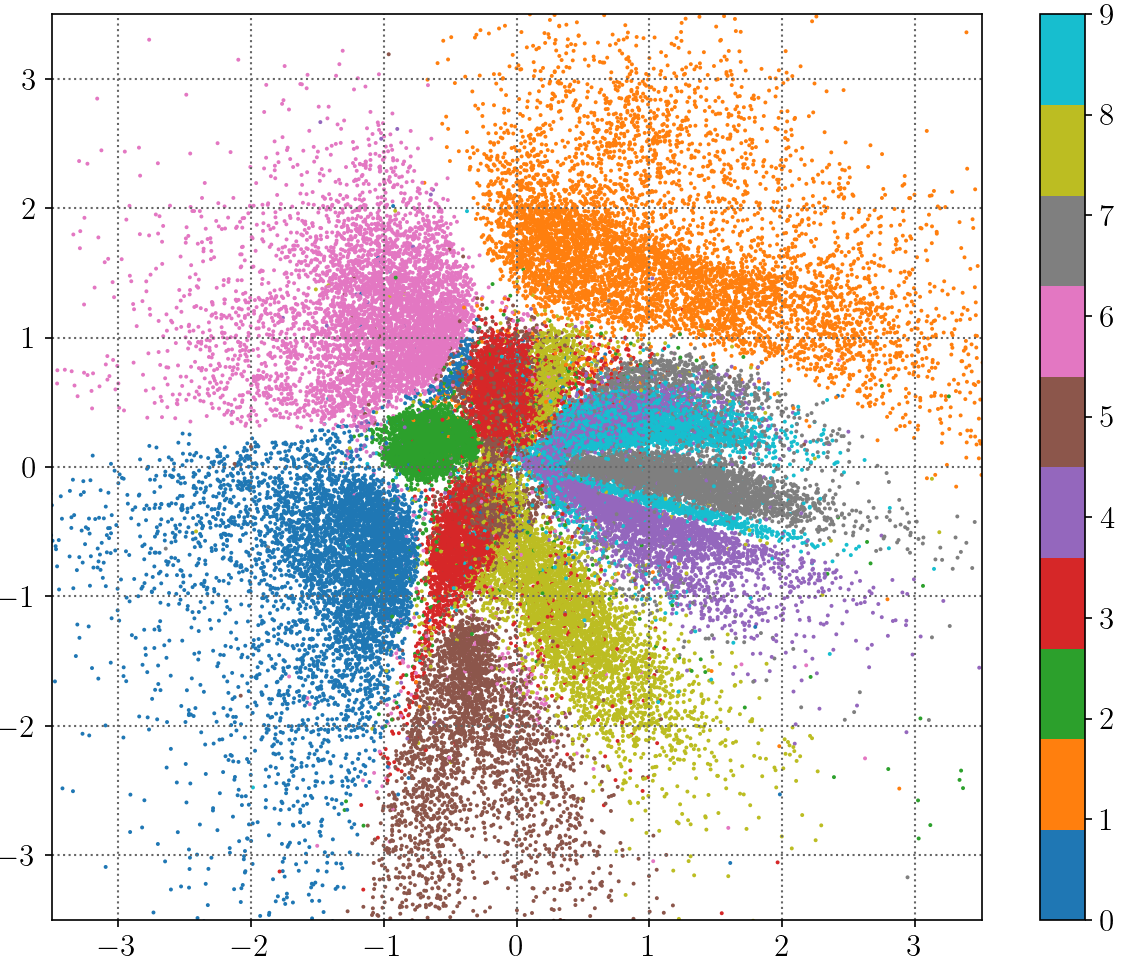
\includegraphics[scale=0.43]{latent_space_2D}
	\end{minipage}%
	\begin{minipage}{.5\textwidth}
		\centering
		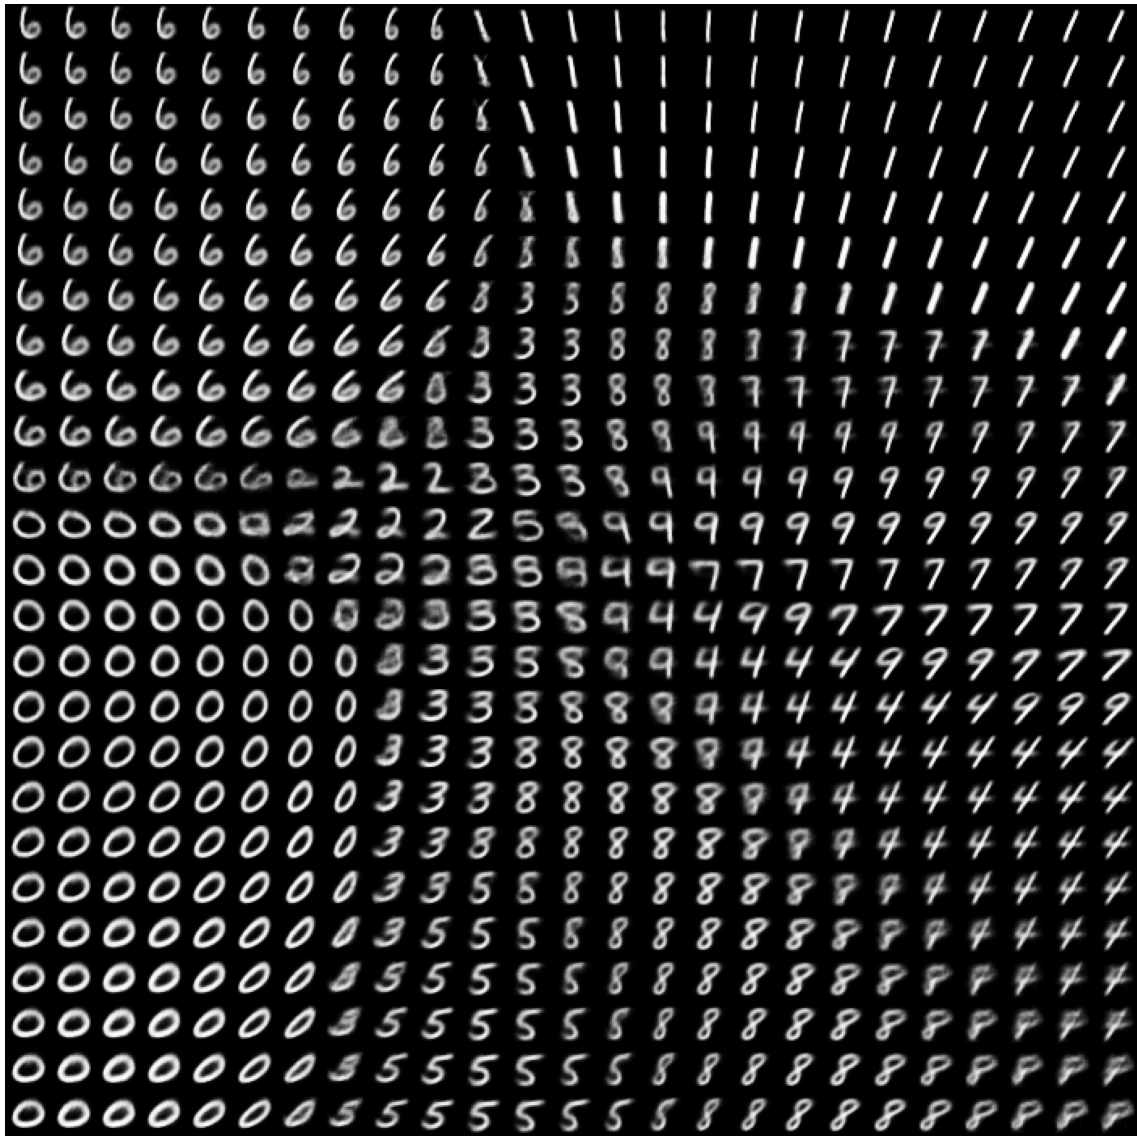
\includegraphics[scale=0.36]{latent_space_2D_reconstructions}
	\end{minipage}
	\captionsetup{labelformat=empty}
	\caption{Erlernte latente Darstellung des MNIST-Trainingsdatensatzes im zweidimensionalen\\ latenten Raum (links) und durch das Decodernetzwerk erzeugte Daten. (rechts) Die \\latenten Darstellungen $\mathbf{z}$ wurden mit linearem Abstand im Quadrat $[-2,2]^2$ gewählt. Auf die verwendete Modellstruktur und den dazu geschriebenen Code gehen wir im praktischen Teil dieser Arbeit genauer ein. } 
	\end{figure}
	Für eine konkrete Berechnung der ELBO betrachten wir zuerst die KL-Divergenz der nun parameterfreien Verteilung $p(\textbf{z})$ nach $q_{\boldsymbol\phi}(\textbf{z}|\textbf{x}_{i})$. $Z$ notiert hierbei die Dimension der latenten Darstellung und $p_{\mathcal{N}(\boldsymbol\mu_{i},\boldsymbol\sigma_{i}^{2}\mathbf{I})}(\textbf{z})$ bzw. $p_{\mathcal{N}(\mathbf{0},\mathbf{I})}(\textbf{z})$ die Auswertung der jeweiligen Dichtefunktion an der Stelle $\textbf{z}$.

	\begin{align*}
	D_{KL}\big(q_{\boldsymbol\phi}(\textbf{z}|\textbf{x}_{i}) || p(\textbf{z})\big) &= \mathbb{E}_{\z\sim\mathcal{N}(\boldsymbol\mu_{i},\boldsymbol\sigma_{i}^{2}\mathbf{I})}\left[\log\left(\frac{p_{\mathcal{N}(\boldsymbol\mu_{i},\boldsymbol\sigma_{i}^{2}\mathbf{I})}(\textbf{z})}{p_{\mathcal{N}(\mathbf{0},\mathbf{I})}(\textbf{z})}\right)\right].\\
	&= \mathbb{E}_{\z\sim\mathcal{N}(\boldsymbol\mu_{i},\boldsymbol\sigma_{i}^{2}\mathbf{I})}\big[\log\big(p_{\mathcal{N}(\boldsymbol\mu_{i},\boldsymbol\sigma_{i}^{2}\mathbf{I})}(\textbf{z})\big)
	- \log\big(p_{\mathcal{N}(\mathbf{0},\mathbf{I})}(\textbf{z})\big)\big].
	\end{align*}
	Die jeweiligen Dichtefunktionen sind durch
	\begin{align*}
	p_{\mathcal{N}(\boldsymbol\mu_{i},\boldsymbol\sigma_{i}^{2}\mathbf{I})}(\textbf{z})&= \frac{1}{\sqrt{2\pi^{Z} \det(\boldsymbol\sigma_{i}^{2}\mathbf{I})}}\exp\left(-\frac{1}{2}(\textbf{z}-\boldsymbol\mu_{i})^{\mathsf{t}}(\boldsymbol\sigma_{i}^{2}\mathbf{I})^{-1}(\textbf{z}-\boldsymbol\mu_{i})\right) \notag \\
	\log(p_{\mathcal{N}(\boldsymbol\mu_{i},\boldsymbol\sigma_{i}^{2}\mathbf{I})}(\textbf{z}))&= -\frac{1}{2}\big(\log(2\pi^{Z} \det(\boldsymbol\sigma_{i}^{2}\mathbf{I}))+(\textbf{z}-\boldsymbol\mu_{i})^{\mathsf{t}}(\boldsymbol\sigma_{i}^{2}\mathbf{I})^{-1}(\textbf{z}-\boldsymbol\mu_{i})\big)\\ \notag 
	\log(p_{\mathcal{N}(\mathbf{0},\mathbf{I})}(\textbf{z}))&= -\frac{1}{2}\left(\log(2\pi^{Z} )+\textbf{z}^{\mathsf{t}}\mathbf{I}\textbf{z}\right)
	\end{align*}
	gegeben. Einsetzen und aufteilen des Erwartungswertes liefert uns
	\begin{align*}
	&\mathbb{E}_{\z\sim\mathcal{N}(\boldsymbol\mu_{i},\boldsymbol\sigma_{i}^{2}\mathbf{I})}\Big[-\frac{1}{2}\Big(\log\big(\det(\boldsymbol\sigma_{i}^{2}\mathbf{I})\big)+(\textbf{z}-\boldsymbol\mu_{i})^{\mathsf{t}}(\boldsymbol\sigma_{i}^{2}\mathbf{I})^{-1}(\textbf{z}-\boldsymbol\mu_{i})-\textbf{z}^{\mathsf{t}}\mathbf{I}\textbf{z}\Big)\Big]\\
	=
	&-\frac{1}{2}\Big(\log\big(\det(\boldsymbol\sigma_{i}^{2}\mathbf{I})\big)+\mathbb{E}_{\z\sim\mathcal{N}(\boldsymbol\mu_{i},\boldsymbol\sigma_{i}^{2}\mathbf{I})}\big[(\textbf{z}-\boldsymbol\mu_{i})^{\mathsf{t}}(\boldsymbol\sigma_{i}^{2}\mathbf{I})^{-1}(\textbf{z}-\boldsymbol\mu_{i})\big]-\mathbb{E}_{\z\sim\mathcal{N}(\boldsymbol\mu_{i},\boldsymbol\sigma_{i}^{2}\mathbf{I})}\big[\textbf{z}^{\mathsf{t}}\mathbf{I}\textbf{z}\big]\Big).
	\end{align*}
	Da $\z\sim\mathcal{N}(\boldsymbol\mu_{i},\boldsymbol\sigma_{i}^{2})$ gilt für die Quadratischen Formen \cite{matrix}:
	\begin{align*}
	\mathbb{E}_{\z\sim\mathcal{N}(\boldsymbol\mu_{i},\boldsymbol\sigma_{i}^{2}\mathbf{I})}\big[\textbf{z}^{\mathsf{t}}\mathbf{I}\textbf{z}\big] &= \boldsymbol\mu_{i}^{\mathsf{t}}\mathbf{I}\boldsymbol\mu_{i}+\mathrm{tr}(\boldsymbol\sigma_{i}^{2}\mathbf{I})\\ \mathbb{E}_{\z\sim\mathcal{N}(\boldsymbol\mu_{i},\boldsymbol\sigma_{i}^{2}\mathbf{I})}\big[(\textbf{z}-\boldsymbol\mu_{i})^{\mathsf{t}}(\boldsymbol\sigma_{i}^{2}\mathbf{I})^{-1}(\textbf{z}-\boldsymbol\mu_{i})\big] &= \mathrm{tr}((\boldsymbol\sigma_{i}^{2}\mathbf{I})^{-1}\boldsymbol\sigma_{i}^{2}\mathbf{I}).
	\end{align*}

	
	Nun lässt sich mit ${\boldsymbol\sigma_{i}^{2}\mathbf{I}} =  \begin{psmallmatrix}\sigma_{i,1}^{2} & \ &\ \\ \ & \ddots &\ \\ \ & \ &\sigma_{i,Z}^{2}\end{psmallmatrix}$ die KL-Divergenz ausrechnen.
	\begin{align*}
	&-\frac{1}{2}\Big(\log\big(\det(\boldsymbol\sigma_{i}^{2}\mathbf{I})\big)+\mathrm{tr}((\boldsymbol\sigma_{i}^{2}\mathbf{I})^{-1}\boldsymbol\sigma_{i}^{2}\mathbf{I})-\boldsymbol\mu_{i}^{\mathsf{t}}\textbf{I}\boldsymbol\mu_{i}-\mathrm{tr}(\boldsymbol\sigma_{i}^{2}\mathbf{I})\Big) \notag \\
	= &-\frac{1}{2}\left(\log\Big(\prod_{j=1}^{Z}\sigma_{i,j}^{2}\Big)+Z-\sum_{j=1}^{Z}\mu_{i,j}^{2}-\sum_{j=1}^{Z}\sigma_{i,j}^{2}\right) \notag \\
	= &-\frac{1}{2}\sum_{j=1}^{Z}\Big(\log\big(\sigma_{i,j}^{2}\big)+1-\mu_{i,j}^{2}-\sigma_{i,j}^{2}\Big).
	\end{align*}
	
	Auch $\pdec$ kann mit unserer Wahl der Verteilungen explizit ausgerechnet werden.
	Mit $P$ wird dazu die Dimension des Inputs und Outputs notiert.
	Für die Verwendung einer multivariaten Normalverteilung im Decoder ergibt sich:
	\begin{align*}
	\log\big(\pdec)\big) &=  \log\big(p_{\mathcal{N}(\boldsymbol{\hat{\mu}}_{i},\boldsymbol{\hat{\sigma}}_{i}^{2}\textbf{I})}(\textbf{x}_{i})\big)\notag \\
	&= -\frac{1}{2}\left(\log(2\pi^{P} \det(\boldsymbol{\hat{\sigma}}_{i}^{2}\textbf{I}))+(\textbf{x}_{i}-\boldsymbol{\hat{\mu}}_{i})^{\mathsf{t}}(\boldsymbol{\hat{\sigma}}_{i}^{2}\textbf{I})^{-1}(\textbf{x}_{i}-\boldsymbol{\hat{\mu}}_{i})\right) \notag \\
	&= -\frac{1}{2}\left(\log(2\pi^{P})+\log\Big( \prod_{p=1}^{P}\hat{\sigma}_{i,p}^{2}\Big)+  \begin{pmatrix}  \frac{x_{i,1}-\hat{\mu}_{i,1}}{\hat{\sigma}_{i,1}^{2}}&\cdots& \frac{x_{i,P}-\hat{\mu}_{i,P}}{\hat{\sigma}_{i,P}^{2}}\end{pmatrix} 
	\boldsymbol{\cdot}(\textbf{x}_{i}-\boldsymbol{\hat{\mu}}_{i})\right) \notag \\
	&= -\frac{1}{2}\left(P\log(2\pi)+\sum_{p=1}^{P}\log\left( \hat{\sigma}_{i,p}^{2}\right)+ 
	\sum_{p=1}^{P}\frac{\big(x_{i,p}-\hat{\mu}_{i,p}\big)^{2}}{\hat{\sigma}_{i,p}^{2}}\right) \notag \\
	&= -\frac{1}{2}\sum_{p=1}^{P} \left(\log\left(2\pi \hat{\sigma}_{i,p}^{2}\right) + \frac{\big(x_{i,p}-\hat{\mu}_{i,p}\big)^{2}}{\hat{\sigma}_{i,p}^{2}}\right)
	\end{align*}
	
	Für eine bernoulliverteilte Zufallsvariable ist die Dichtefunktion  durch $p_{\mathcal{B}(\mathrm{p}_{i})}(x_{i}) = \mathrm{p}_{i}^{x_{i}}(1-\mathrm{p}_{i})^{(1-x_{i})}$ definiert. Somit ergibt sich für die Verwendung der multivariaten Bernoulliverteilung im Decoder: \\
	\begin{align*}
	\log\big(p_{\theta}(\textbf{x}_{i}|\textbf{z})\big) &=  \log\big(p_{\mathcal{B}(\boldsymbol{p}_{i})}(\textbf{x}_{i})\big)\notag \\
	&= \log\left(p_{\mathcal{B}(\mathrm{p}_{1})}\left(x_{i,1}\right)\ \cdot\ldots\cdot \ p_{\mathcal{B}(\mathrm{p}_{P})}\left(x_{i,P}\right)\right)\notag \\
	&= \log\left(\prod_{p=1}^{P}\left(p_{i,p}\right)^{x_{i,p}}\left(1-p_{i,p}\right)^{\left(1-x_{i,p}\right)}\right) \notag \\
	&=  \sum_{p=1}^{P}x_{i,p}\log\left(p_{i,p}\right)+\left(1-x_{i,p}\right)\log\left(1-p_{i,p}\right)
	\end{align*}			
	\subsection[ODE$^2$-VAE]{Ordinary Differential Equation Variational Autoencoder}
	Als Trainingskriterium des ODE$^2$-VAE verwenden wir erneut die ELBO (eine genauere Erklärung ist im Kapitel zum VAE zu finden). 
	Wir erhalten:
	\begin{align*}
	\log\left(\mathbf{x}_{0:T}\right)&\ge \E_{\mathbf{z}_{0:T}\sim q_{\boldsymbol\phi,\boldsymbol\psi}}
	\left[\log\left(p_{\boldsymbol\theta}\left(\mathbf{x}_{0:T}|\mathbf{z}_{0:T}\right)\right)\right] - D_{KL}\big[q_{\boldsymbol\phi,\boldsymbol\psi}(\mathbf{z}_{0:T}|\mathbf{x}_{0:m})||p_{\boldsymbol\theta,\boldsymbol\psi}(\mathbf{z}_{0:T})\big]\\
	&=\underbrace{\E_{\mathbf{z}_{0}\sim q_{\text{enc }\boldsymbol\phi}}
	\left[\log\left(p_{\boldsymbol\theta}\left(\mathbf{x}_{0}|\mathbf{z}_{0}\right)\right)\right] - D_{KL}\big[q_{\text{enc }\boldsymbol\phi}(\mathbf{z}_{0}|\mathbf{x}_{0:m})||p_{\boldsymbol\theta}(\mathbf{z}_{0})\big]}_{\text{Vanilla-VAE ELBO}}\\ &+ \underbrace{\sum_{t=1}^T \E_{\mathbf{z}_{t}\sim q_{\text{flow }\boldsymbol\psi}}
	\left[\log\left(p_{\boldsymbol\theta}\left(\mathbf{x}_{t}|\mathbf{z}_{t}\right)\right)\right] - D_{KL}\big[q_{\text{flow }\boldsymbol\psi}(\mathbf{z}_{t}|\mathbf{x}_{0:m})||p_{\boldsymbol\theta,\boldsymbol\psi}(\mathbf{z}_{t})\big]}_{\text{Dynamischer Loss}}
	\end{align*}	
	Der erste Teil ist die ELBO eines Standard-VAEs.
	Als dem latenten Raum zugrundeliegenden Verteilung $p_{\boldsymbol\theta}(\mathbf{z}_{0})$ wählen wir erneut eine parameterfreie Standardnormalverteilung $\mathcal{N}(\mathbf{0},\mathbf{I})$.\\
	Die Encoder-Verteilung ist als Normalverteilung mit $\mathbf{z}_{0} = (\mathbf{s}_{0},\mathbf{v}_{0})^t$ durch
	\begin{align*}
	q_{\text{enc }\boldsymbol\phi}(\mathbf{z}_{0}|\mathbf{x}_{0:m}) =	 
	\mathcal{N}\left(\left(\begin{array}{cc} 
	\boldsymbol\mu_{\text{pos }\boldsymbol\phi}(\textbf{x}_{0}) \\ 
	\boldsymbol\mu_{\text{vel }\boldsymbol\phi}(\textbf{x}_{0:m}) 
	\end{array}\right),\left(\begin{array}{cc} 
	\text{diag}(\boldsymbol\sigma_{\text{pos }\boldsymbol\phi}(\textbf{x}_{0})) & 
	\mathbf{0}\\ 
	\mathbf{0} & 
	\text{diag}(\boldsymbol\sigma_{\text{vel }\boldsymbol\phi}(\textbf{x}_{0:m}))  
	\end{array}\right)\right)
	\end{align*}	
	gegeben. Wie erläutert hängt der Output des Velocity-Encoders dabei von den ersten $m\ge3$ Zuständen ab, während der Output des Position-Encoders nur durch den ersten Zustand bestimmt wird.\\
	Die Berechnung des Reconstruction Loss ist von der Wahl der im Decoder verwendeten Verteilung abhängig.
	Die analytische Berechnung ist nun mit den Resultaten des letzten Kapitels möglich. (S.XYZ)\\  
	Die Berechnung des sogenannten Dynamischen Loss ist komplizierter.
	Der Reconstruction Loss $\E_{\mathbf{z}_{t}\sim q_{\text{flow }\boldsymbol\psi}}
	\left[\log\left(p_{\boldsymbol\theta}\left(\mathbf{x}_{t}|\mathbf{z}_{t}\right)\right)\right] $ lässt sich zwar ebenfalls mit den Resultaten des ersten Kapitels berechnen. (S.XYZ) \\
	Für die approximative Berechnung KL-Divergenz 
	\begin{align*}
	D_{KL}\big[q_{\text{flow }\boldsymbol\psi}(\mathbf{z}_{t}|\mathbf{x}_{0:m})||p_{\boldsymbol\theta,\boldsymbol\psi}(\mathbf{z}_{t})\approx \log\left(q_{\text{flow }\boldsymbol\psi}(\mathbf{z}_{t}|\mathbf{x}_{0:m}) \right) - \log\left(p_{\boldsymbol\theta,\boldsymbol\psi}(\mathbf{z}_{t}) \right)
	\end{align*}
	benötigen wir jedoch die Dichten der Flow-Verteilung $q_{\text{flow }\boldsymbol\psi}(\mathbf{z}_{t}|\mathbf{x}_{0:m})$ und die der Prior-Verteilung $p_{\boldsymbol\theta,\boldsymbol\psi}(\mathbf{z}_{t})$.\\
	Die latenten Werte $\mathbf{z}_{t} = (\mathbf{s}_{t},\mathbf{v}_{t})^t$ sind nun nicht mehr von den Encoder-Netzwerken abhängig, sondern werden durch die Neuronale Differentialgleichung $f_{\boldsymbol\psi}(\mathbf{s}_{t},\mathbf{v}_{t})$ bestimmt. 
	Zur Berechnung der Dichte der Flow-Verteilung lassen sich folgende hilfreiche Theoreme anwenden.
	\begin{theorem}
	Sei $\mathbf{z}(t)$ eine stetige Zufallsvariable mit einer von der Zeit abhängigen Dichtefunktion $q(\mathbf{z}(t))$. Sei $\tfrac{\partial \mathbf{z}(t)}{\partial t}=f(\mathbf{z}(t),t)$ eine in $\mathbf{z}$ Lipschitzstetige und in $t$ stetige Differentialgleichung, welche die Veränderung von $\mathbf{z}(t)$ mit der Zeit beschreibt.
	Die Veränderung der Dichte folgt nun ebenfalls einer Differentialgleichung:
	\begin{align*}
	\dfrac{\partial \log\left(q(\mathbf{z}(t)\right)}{\partial t}&= - \mathrm{Tr}\left(\dfrac{\partial f}{\partial\mathbf{z}}(t)\right).
	\end{align*}
	\end{theorem}
	\begin{proof}
	Zu finden in \emph{Neural Ordinary Differential Equations} \cite{neuralode}, S.13
	\end{proof}
		\begin{theorem}%{$\mathrm{(Hutchinsons\ Spur\ Schätzer)}$}
		Sei $\mathbf{M}\in \mathbb{R}^d \times \mathbb{R}^d$ eine beliebige Matrix und $\boldsymbol\epsilon \sim p(\boldsymbol\epsilon)$ eine Zufallsvariable mit $\E[\boldsymbol\epsilon] = \mathbf{0}$ und $Cov(\boldsymbol\epsilon) =\mathbf{I}$. Die Spur der Matrix $\mathbf{M}$ lässt sich erwartungstreu durch ein doppeltes Matrix-Vektorprodukt der Matrix  $\mathbf{M}$ mit dem Zufallvektor $\boldsymbol\epsilon$ schätzen:
		\begin{align*}
		\mathrm{Tr}(\mathbf{M}) = 
		\E_{\boldsymbol\epsilon \sim p(\boldsymbol\epsilon)}\big[\boldsymbol\epsilon^t \mathbf{M} \boldsymbol\epsilon \big].
		\end{align*}
	\end{theorem}
	\begin{proof}
		TO-DO %http://blog.shakirm.com/2015/09/machine-learning-trick-of-the-day-3-hutchinsons-trick/
	\end{proof}
	
	Wir erhalten somit für die Veränderung der Log-Dichte der Flow-Verteilung:
	\begin{align*}
	\dfrac{\partial \log\left(q_{\text{flow }\boldsymbol\psi}(\mathbf{z}_{t}|\mathbf{x}_{0:m})\right)}{\partial t}\overset{\text{T.1}}&{=} - \text{Tr}\left(\dfrac{\partial f_{\boldsymbol\phi}(\mathbf{z}_{t})}{\partial\mathbf{z}_{t}}\right) \\ &=
	- \text{Tr} \left(\begin{array}{cc} 
	\dfrac{\partial\mathbf{v}_{t}}{\partial\mathbf{s}_{t}} & 
	\dfrac{\partial\mathbf{s}_{t}}{\partial\mathbf{v}_{t}}\\ 
	\dfrac{\partial f_{\boldsymbol\phi}(\mathbf{s}_{t},\mathbf{v}_{t})}{\partial\mathbf{s}_{t}} & 
	\dfrac{\partial f_{\boldsymbol\phi}(\mathbf{s}_{t},\mathbf{v}_{t})}{\partial\mathbf{v}_{t}}  
	\end{array}\right)\\
	&=
	-\text{Tr}\left(\dfrac{\partial f_{\boldsymbol\phi}(\mathbf{s}_{t},\mathbf{v}_{t})}{\partial\mathbf{v}_{t}}\right)\\
	\overset{\text{T.2}}&{=} \E_{\boldsymbol\epsilon\sim\mathcal{N}(0,\text{I})}\left[\boldsymbol\epsilon^\mathrm{t}\dfrac{\partial f_{\boldsymbol\phi}(\mathbf{z}_{t})}{\partial\mathbf{v}_{t}}\boldsymbol\epsilon\right].
	\end{align*}		
	Durch Integration ergibt sich nun:
	\begin{align*}
	\log\left(q_{\text{flow }\boldsymbol\psi}(\mathbf{z}_{t}|\mathbf{x}_{0:m})\right)&=\log\left(q_{\text{enc }\boldsymbol\phi}(\mathbf{z}_{0}|\mathbf{x}_{0:m})\right)-\int_0^t \E_{\boldsymbol\epsilon\sim\mathcal{N}(0,\text{I})}\left[\boldsymbol\epsilon^\mathrm{t}\dfrac{\partial f_{\boldsymbol\phi}(\mathbf{s}_{t},\mathbf{v}_{t})}{\partial\mathbf{v}_{t}}\boldsymbol\epsilon\right]\text{d}t\\
	&= \log\left(q_{\text{enc }\boldsymbol\phi}(\mathbf{z}_{0}|\mathbf{x}_{0:m})\right)-\E_{\boldsymbol\epsilon\sim\mathcal{N}(0,\text{I})}\left[\int_0^t \boldsymbol\epsilon^\mathrm{t}\dfrac{\partial f_{\boldsymbol\phi}(\mathbf{s}_{t},\mathbf{v}_{t})}{\partial\mathbf{v}_{t}}\boldsymbol\epsilon\ \text{d}t\right].
	\end{align*}		
	
	\subsection[SDE-VAE]{Stochastic Differential Equation Variational Autoencoder}

	
	\section[Empirische Untersuchung]{Empirische Untersuchung}
	\subsection[VAE]{Ergebnisse: VAE}
	
	\textbf{TODO: Bild einfügen VAE Rekonstruktion ohne Interpolation}
	\begin{figure}[!htbp]
		\centering
%		\includegraphics[scale=1]{DreieckLemma}
		\caption{Rekonstruktion der \emph{time series} mittels VAE ohne Interpolation.}
	\end{figure}
	\textbf{TODO: Bild einfügen VAE Rekonstruktion mit Interpolation}
	\begin{figure}[!htbp]
		\centering
		%		\includegraphics[scale=1]{DreieckLemma}
		\caption{Rekonstruktion der \emph{time series} mittels VAE mit Interpolation.}
	\end{figure}
	\newpage
	\subsection[ODE$^2$-VAE]{Ergebnisse: ODE$^2$-VAE}

	%\begin{figure}
	%	\begin{minipage}[position=l]{0.33\textwidth}
	%		\begin{mdframed}[style=inner]
	%			\center{Modellinput\vspace{0.2cm}}
	%			
\includegraphics[scale=0.5]{Modellinput}
	%		\end{mdframed}
	%	\end{minipage}
	%	\begin{minipage}[position=r]{0.67\textwidth}
	%		\begin{mdframed}[style=inner]
	%			\center{Rekonstruktionen\vspace{0.2cm}}
	%%			\includegraphics[scale=0.499]{Reconstructions}
	%		\end{mdframed}
	%	\end{minipage}
	%\caption{Groundtruth (jeweils obere Reihe) und Rekonstruktionen des ODE$^2$-VAE (untere %Reihe) auf den Testdatensätzen von Rotating MNIST und Bouncing Balls. Wie erwähnt erhält das %Modell nur die ersten drei Bilder der \emph{time series}, um Vorhersagen für die restlichen %Zeitpunkte zu treffen.}
%	\end{figure}
	\newpage
	\subsection[SDE-VAE]{Ergebnisse: SDE-VAE}
	\newpage
	\section[Code]{Code}
	
	\section[Quellenangabe]{Quellenangabe}
	\begin{thebibliography}{9}
		\bibitem{vae}
		Diederik P. Kingma, Max Welling,
		\textit{Auto-Encoding Variational Bayes},
		2013,\\
		arXiv:1312.6114v10
		
		\bibitem{intvae}
		Diederik P. Kingma, Max Welling,
		\textit{An Introduction to Variational Autoencoders}, 
		2019,
		arXiv:1906.02691v3
		
		\bibitem{ode2vae}
		Çağatay Yıldız, Markus Heinonen, Harri Lähdesmäki,
		\textit{ODE$^{\ 2}$-VAE: Deep generative second order ODEs with Bayesian neural networks}, 
		2019,
		arXiv:1905.10994v2
		
		\bibitem{repara}
		https://gabrielhuang.gitbooks.io/machine-learning/content/reparametrization-trick.html

		\bibitem{tutvae}
		Carl Doersch,
		\textit{Tutorial on Variational Autoencoders},
		2016,\\
		arXiv:1606.05908,
		Ähnliche Grafik zu finden auf S.5

		\bibitem{matrix}
		Kaare B. Petersen, Michael S. Pedersen,
		\textit{The Matrix Cookbook},
		2012,
		http://matrixcookbook.com, Verwendete Rechentricks auf S.43
		
		\bibitem{neuralode}
		Ricky T. Q. Chen, Yulia Rubanova, Jesse Bettencourt, David Duvenaud,\\
		\textit{Neural Ordinary Differential Equations},
		2019, arXiv:1806.07366v5

	\end{thebibliography}
	\section[Anhang]{Anhang}
	\subsection[Analytische Berechnung der ELBO]{Analytische Berechnung der ELBO}
	\subsection[Analytische Berechnung der Lossfunktion des ODE$^2$-VAE]{Analytische Berechnung der Lossfunktion des ODE$^2$-VAE}
\end{document}
